This appendix examines the $\pod$-only BANFF fit likelihood term
$\chi_{\text{LLR}}^{2}=\chi_{\text{sample}}^{2}$ response (scans)
to variations in flux and cross section parameters. For the cross
section terms, the scans shapes correspond to the shape of the spline
weight. In addition, comparison scans are provided for the FGD MaCH3
2017 analysis. Extensive comparisons were made to ensure that the
FGD MaCh3 and FGD BANFF analyses have identical splines. So it is
an equal comparison with the FGD BANFF as shown in \prettyref{chap:P0DinBANFF}.
In some cases, the $\pod$-only scans indicate higher sensitivity
to parameters than the FGD.

These were generously produced by Clarence Wret (c.wret@rochester.edu)
of the University of Rochester. The likelihood scans are ordered as
such. The first 50 plots ``b\_0\_sam'' through ``b\_49\_sam''
are the ND280 flux sample contributions. The next 50 ``b\_50\_sam''
through ``b\_99\_sam'' are the sample contributions that affect
the SK flux. The last scans are variations on the cross section parameters.
Due to a bug in plotting script, the scans 2p2h shape location for
\ce{^{12}C} and \ce{^{16}O} were empty for the $\pod$. The correct
$\pod$ scans are shown in \prettyref{fig:Correct-shape-scans} with
the MaCH3 inputs reproduced as faithfully as possible.

As expected, the SK flux variations are flat with respect to the sample
chi-squared. This is due model parameterization in which the ND280
samples only affect the ND280 flux parameters. In other words, the
log-likelihood scans for the SK flux parameters have no affect on
the ND280 sample events.

Some of cross section parameter splines are reflected about a point
in order to properly calculate correlations between parameters. In
previous fits to data, the 2p2h \ce{^{12}C} and \ce{^{16}O} shape
location terms hit their physical boundaries at +1. The result was
that the fitter MINUIT inaccurately calculated the Hess matrix. The
decision was made to reflect, also called ``mirroring'', the splines
about a certain point to expand the limit. Tests showed that this
did not affect the postfit results for any parameters, but the correlations
between all other parameters was calculated to less than 1\%\cite{Bienstock2017}.

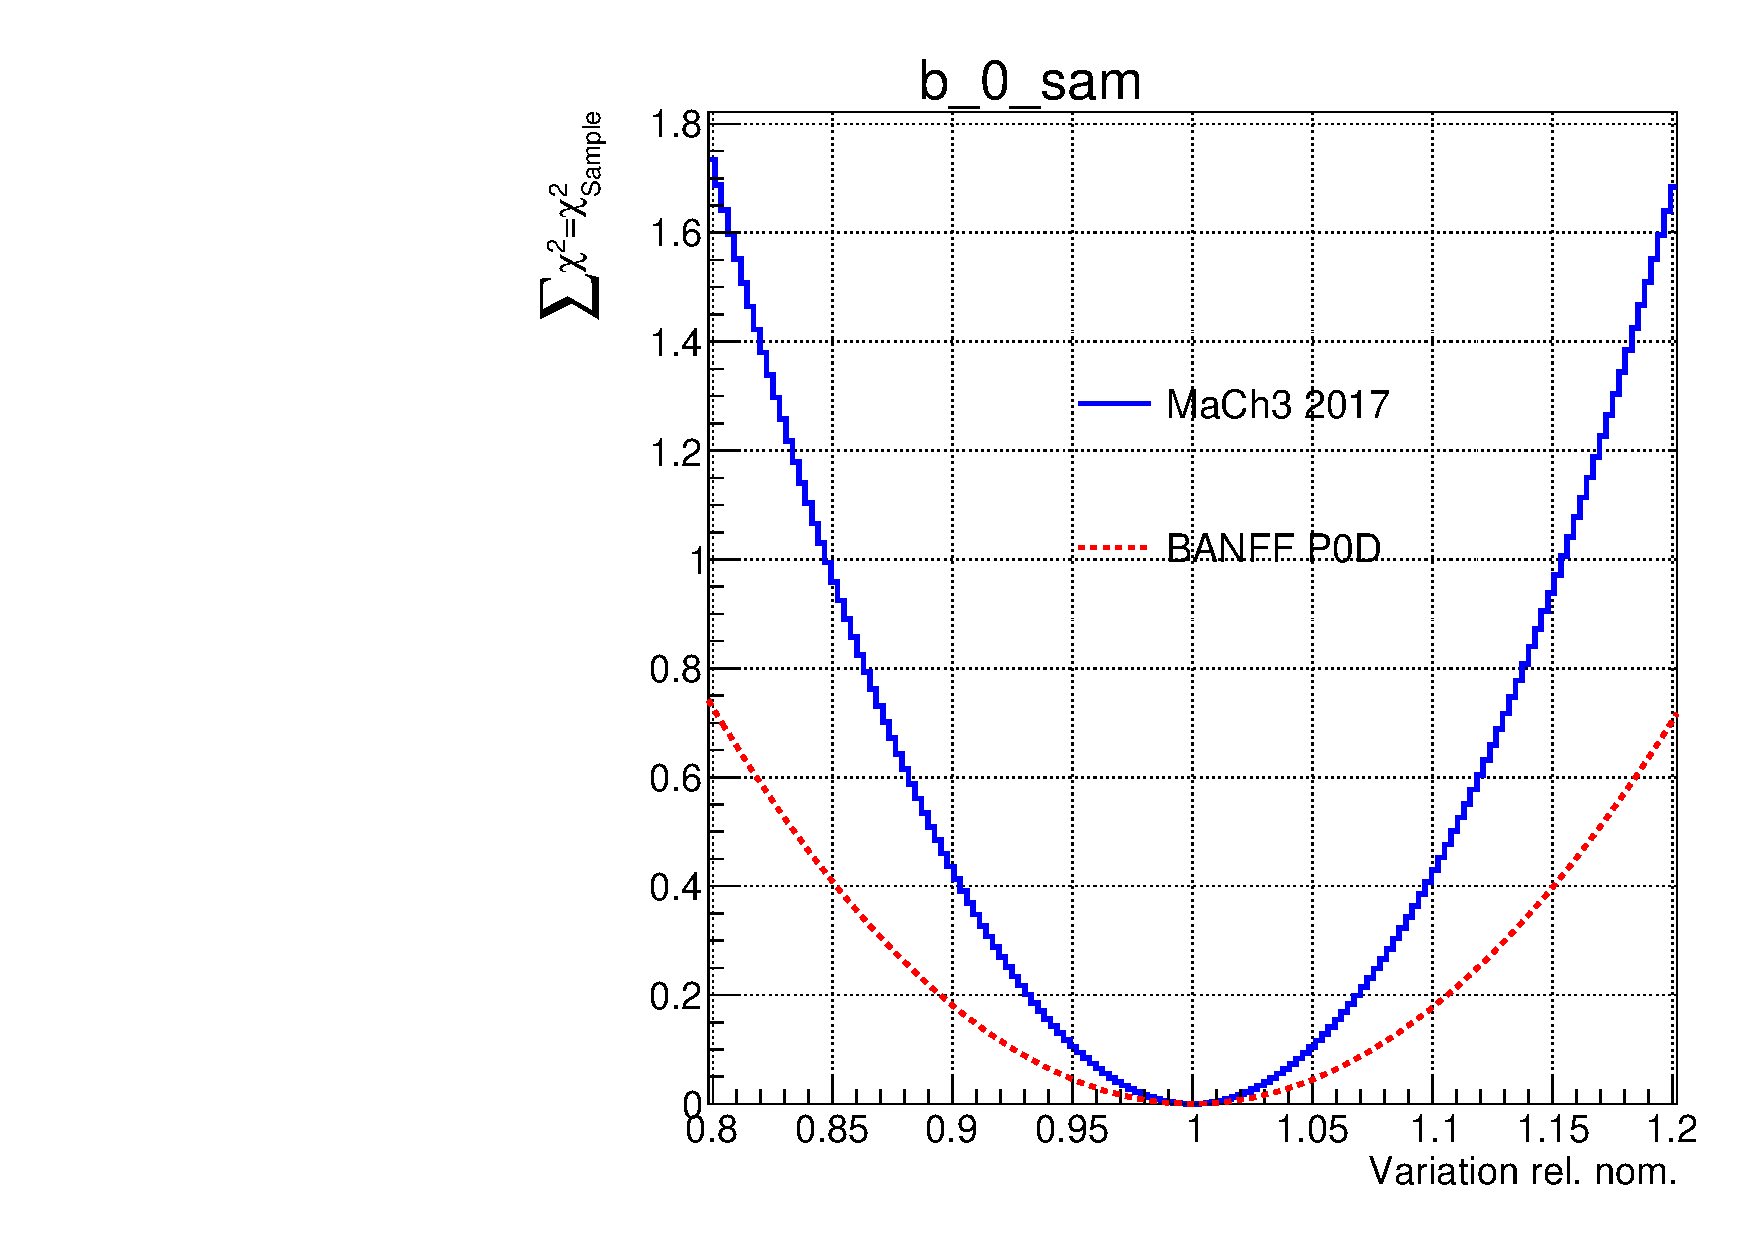
\includepdf[nup=3x4,pages={1-129},pagecommand=\thispagestyle{plain},width=2in]{Appendices/Figures/LikeLihoodScans/p0d_vs_mach3_sample}

\begin{figure}
\begin{centering}
\subfloat[]{\begin{centering}
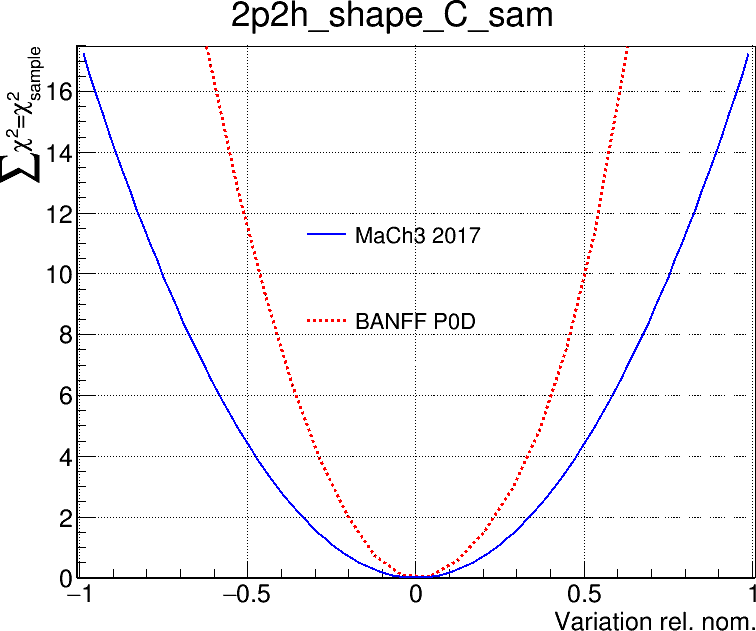
\includegraphics[width=0.45\textwidth]{Appendices/Figures/LikeLihoodScans/2p2h_shape_C_sam}
\par\end{centering}

}\subfloat[]{\begin{centering}
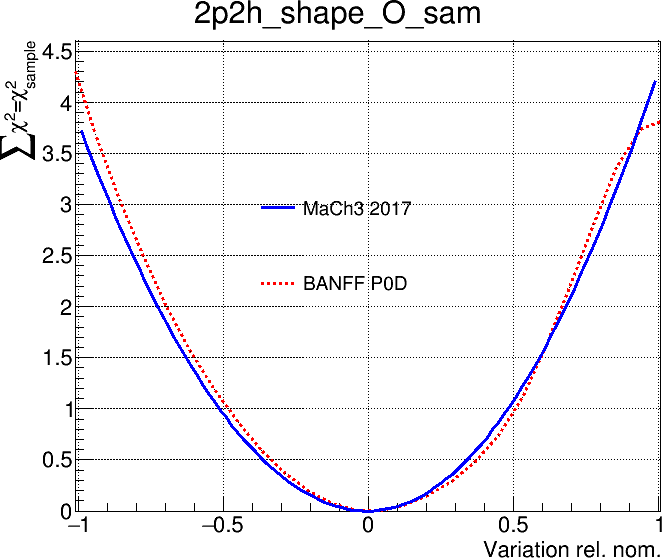
\includegraphics[width=0.45\textwidth]{Appendices/Figures/LikeLihoodScans/2p2h_shape_O_sam}
\par\end{centering}
}
\par\end{centering}
\caption[Corrected 2p2h Shape Location Scans]{Correct $\pod$ scans with faithful reproductions of the MaCh3 scans
for the 2p2h shape location cross section parameters.\label{fig:Correct-shape-scans}}

\end{figure}

